\section{Unions}

\begin{frame}[fragile]{Unions}
	\begin{itemize}
		\item Bekannt: \verb|class| und \verb|struct|
		\begin{itemize}
			\item Fassen Daten (Member) und Methoden zusammen
			\item Das ganze ist (mehr als) die Summe seiner Teile
		\end{itemize}
		\pause
		\item Neu: \verb|union|
		\begin{itemize}
			\item NICHT die Summe aller Teile, KEIN Aggregat
			\item Alle deklarierten Member landen an der gleichen Stelle im Speicher
			\item Ein Union kann Daten verschiedenen Typs aufnehmen
			\item Aber zu jedem Zeitpunkt nur von einem Typ
			\item Nutzung wie bei \verb|class| und \verb|struct|: \verb|myUnion.foo = 42|
			\item Möglich: Methoden, \verb|private, protected, public|, Konstruktoren und Destruktoren
			\item Verboten: Jede Form von Vererbung
		\end{itemize}
	\end{itemize}
\end{frame}

\begin{frame}[fragile]{Unions: Vergleich mit Structs}
	\begin{columns}
		\column{.4\textwidth}
			\lstinputlisting[language=C++]{cpp-code/structunion.cpp}
			
		\column{.6\textwidth}
			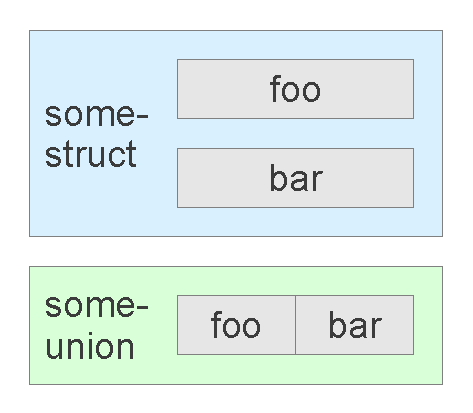
\includegraphics[width=\linewidth]{images/structunion.pdf}
	\end{columns}
\end{frame}

\begin{frame}[fragile]{Unions: Motivation}
	\begin{itemize}
		\item Ursprung: Plain old C, Speicherung verschiedener Typen in einer Variablen
		\begin{itemize}
			\item \enquote{Polymorphismus für Arme}
		\end{itemize}
		\pause
		\item In C++: Auch nur ein Container für verschiedene Typen \dots
		\pause
		\item Type Punning: \verb|foo_t| rein, \verb|bar_t| raus
		\begin{itemize}
			\item Wird NICHT vom Standard gedeckt!
			\item Compilerabhängig
		\end{itemize}
	\end{itemize}
\end{frame}

\begin{frame}[fragile]{Anonyme Unions}
	\begin{itemize}
		\item Unions die selbst nicht in Erscheinung treten/transparent sind
	\end{itemize}
	\begin{columns}
		\column{.45\textwidth}
			\lstinputlisting[language=C++, linerange={1-9}, numbers=left, numberstyle=\tiny\color{gray}]{cpp-code/anonymous.cpp}
			
		\column{.45\textwidth}
			\lstinputlisting[language=C++, linerange={11-19}, numbers=left, numberstyle=\tiny\color{gray}]{cpp-code/anonymous.cpp}
	\end{columns}
\end{frame}

\begin{frame}[fragile]{Unions: Anwendungsbeispiel Variant}
	\lstinputlisting[language=C++]{cpp-code/variant.cpp}
\end{frame}

